%%%%%%%%%%%%%%%%%%%%%%%%%%%%%%%%%%%%%%%%%
% Stylish Article
% LaTeX Template
% Version 2.1 (1/10/15)
%
% This template has been downloaded from:
% http://www.LaTeXTemplates.com
%
% Original author:
% Mathias Legrand (legrand.mathias@gmail.com) 
% With extensive modifications by:
% Vel (vel@latextemplates.com)
%
% License:
% CC BY-NC-SA 3.0 (http://creativecommons.org/licenses/by-nc-sa/3.0/)
%
%%%%%%%%%%%%%%%%%%%%%%%%%%%%%%%%%%%%%%%%%

%----------------------------------------------------------------------------------------
%	PACKAGES AND OTHER DOCUMENT CONFIGURATIONS
%----------------------------------------------------------------------------------------

\documentclass[UTF8, fleqn,10pt]{SelfArx} % Document font size and equations flushed left

\renewcommand{\thefootnote}{\alph{footnote}}
\usepackage[english]{babel} % Specify a different language here - english by default
\usepackage{float}
\usepackage{lipsum} % Required to insert dummy text. To be removed otherwise
\usepackage[space]{ctex} %中文包
%----------------------------------------------------------------------------------------
%	COLUMNS
%----------------------------------------------------------------------------------------

\setlength{\columnsep}{0.55cm} % Distance between the two columns of text
\setlength{\fboxrule}{0.75pt} % Width of the border around the abstract

%----------------------------------------------------------------------------------------
%	COLORS
%----------------------------------------------------------------------------------------

\definecolor{color1}{RGB}{0,0,90} % Color of the article title and sections
\definecolor{color2}{RGB}{0,20,20} % Color of the boxes behind the abstract and headings

%----------------------------------------------------------------------------------------
%	HYPERLINKS
%----------------------------------------------------------------------------------------
\usepackage{algorithm}  
\usepackage{algorithmicx}  
\usepackage{algpseudocode}  
\usepackage{amsmath}  
\floatname{algorithm}{算法}  
\renewcommand{\algorithmicrequire}{\textbf{输入:}}  
\renewcommand{\algorithmicensure}{\textbf{输出:}}  
\usepackage{hyperref} % Required for hyperlinks
\hypersetup{hidelinks,colorlinks,breaklinks=true,urlcolor=color2,citecolor=color1,linkcolor=color1,bookmarksopen=false,pdftitle={Title},pdfauthor={Author}}

%----------------------------------------------------------------------------------------
%	ARTICLE INFORMATION
%----------------------------------------------------------------------------------------
\JournalInfo{2020年春季大数据算法课程结题报告} % Journal information
\Archive{中国科学技术大学} % Additional notes (e.g. copyright, DOI, review/research article)

\PaperTitle{核心向量机的深度研究与创新} % Article title

\Authors{吴颖馨\textsuperscript{1}, 张永停\textsuperscript{2}} % Authors
\affiliation{\textsuperscript{1}\textit{Department of Big Data, USTC. wuyxin@mail.ustc.edu.cn}} % Author affiliation
\affiliation{\textsuperscript{2}\textit{Department of Computer Science, USTC}} % Author affiliation
%\affiliation{*\textbf{Corresponding author}: john@smith.com} % Corresponding author

\Keywords{Keyword1 --- Keyword2 --- Keyword3} % Keywords - if you don't want any simply remove all the text between the curly brackets
\newcommand{\keywordname}{Keywords} % Defines the keywords heading name

%----------------------------------------------------------------------------------------
%	ABSTRACT
%----------------------------------------------------------------------------------------

\Abstract{\lipsum[1]~}

%----------------------------------------------------------------------------------------

\begin{document}

\flushbottom % Makes all text pages the same height

\maketitle % Print the title and abstract box

\tableofcontents % Print the contents section

\thispagestyle{empty} % Removes page numbering from the first page

%----------------------------------------------------------------------------------------
%	ARTICLE CONTENTS
%----------------------------------------------------------------------------------------

\section*{Introduction} % The \section*{} command stops section numbering

\addcontentsline{toc}{section}{Introduction} % Adds this section to the table of contents
\lipsum[1]
%------------------------------------------------

\section{算法详细总结}
以下将对参考文献[1, 2]总结完整的数学推导。为避免本论文对参考文献中推导过程的简单重复,总结将加入对问题的形象叙述与直观理解。考虑到叙述的完整性,1.1节中将简述经典的 SVM,并推导详细的L2 norm soft margin SVM的对偶形式,这将在"Core Vector Machines:
Fast SVM Training on Very Large Data Sets"中用到。1.2节将介绍CVM的主要算法,1.3节将介绍在论文[2]中与CVM进行对比的SimpleSVM算法。1.4节将讨论CVM的收敛性、时空复杂度以及算法上与SimpleSVM的对比(补充)。
	\subsection{Support Vector Machine}
	$SVM$ 适用于非参数线性分类问题,所谓非参数机器学习算法,指的是不对目标函数的形式做太多假设。而在没有假设的情况下,算法可以自由地从训练数据中学习函数的任何形式。$SVM$ 的另外一大优势在于,将其转化为对偶问题后,分类只需计算支持向量机与少数支持向量之间的距离,在计算复杂核函数时可以大大简化模型和计算。
	\begin{figure}[H]
		\centering
		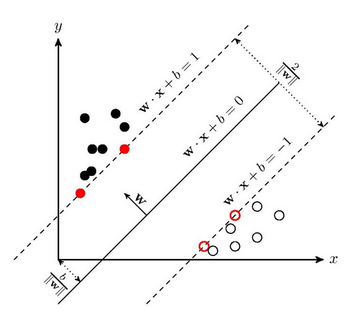
\includegraphics[width=0.3\textwidth]{figure/svm}
		\caption{SVM在二维平面中的表示,通过最大化几何间隔来确定最优划分超平面}
	\end{figure}
	首先,SVM是基于线性可分的数据集 $X$,但是现实世界中,这一假设往往不能被实现。然而可以证明*,$\exists$ 高维度映射 $\phi$, $X \xrightarrow{\phi} \phi(X)$ 使得 $X$ 线性可分。以下直接用 $\phi(X)$ 表示线性可分的数据集。\par
	为最大化几何间隔,并将目标转换为凸函数形式(此处不再赘述),可以得到以下优化形式:
	\begin{equation}
	\begin{aligned}
	&\mathop{min}\limits_{\omega, b} \frac{1}{2} \left\|\omega\right\|^2\\
	&s.t. \   y_{i}(\omega^{T}\phi(x^{(i)})+b) \geq 1,\ i = 1,2,...,m
	\end{aligned}
	\end{equation}
	$y^{(i)}$ 为 第i个节点特征 $x^{(i)}$ 对应的label,$\omega, b$ 为待学习参数。相应的对偶问题为
	\begin{equation}
	\begin{aligned}
	&\mathop{min}\limits_{\alpha} W(\alpha) =\sum_{i=1}^{m} \alpha_{i}-\frac{1}{2}\sum_{i=1}^{m}\sum_{j=1}^{m}\alpha_{i}\alpha_{j}y^{(i)}y^{(j)}\phi(x^{(i)})^{T}\phi(x^{(j)})\\
	&s.t. \   \sum_{i=1}^{m}\alpha_{i}y^{(i)} = 0,\\
	&\alpha_{i} \geq 0,\ i=1, 2, ..., m
	\end{aligned}
	\end{equation}
	\paragraph{Sequential Minimal Optimization}(Platt et al. 1998)被提出以优化该对偶问题,算法思想十分清晰简洁。
	\begin{quote}
		Repeat\{\\
		Select $\alpha_{i},\alpha_{j}$\\
		Hold all $\alpha_{k}$ fixed, except $\alpha_{i},\alpha_{j}$\\
		Optimize W($\alpha$) w.r.t. $\alpha_{i},\alpha_{j}$\\(subject to all the constraints).\\
		\}
	\end{quote}
	\paragraph{L2 Norm Soft Margin SVM}\ 
	\begin{figure}[H]
		\centering
		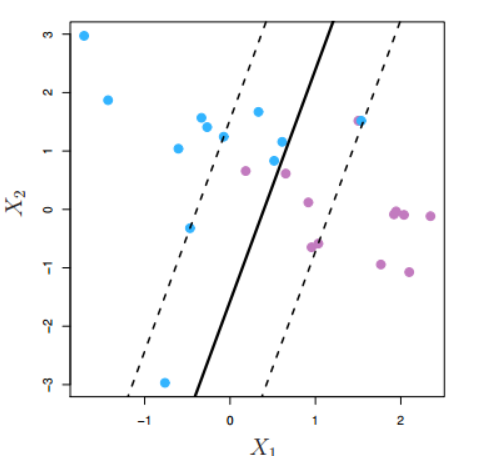
\includegraphics[width=0.3\textwidth]{figure/softsvm}
		\caption{L2 Norm Soft Margin SVM。一方面考虑到数据(即使在高维空间)不一定线性可分,另一方面希望去除部分噪声点。可以形象化描述为“允许但不鼓励一部分点跨过超平面”。}
	\end{figure}
	\noindent
	在L2正则下,我们需要优化的目标为
	\begin{equation*}
	\begin{aligned} \min _{\omega, b, \xi} & \frac{1}{2}\|\omega\|^{2}+\frac{C}{2} \sum_{i=1}^{m} \xi_{i}^{2} \\ \text { s.t. } & y^{(i)}\left(\omega^{T} x^{(i)}+b\right) \geq 1-\xi_{i}, \quad i=1, \ldots, m \end{aligned}
	\end{equation*}
	对上述限制采用拉普拉斯算子重新表述为
	$$
	\mathcal{L}(\omega, b, \xi, \alpha)=\frac{1}{2} \omega^{T} \omega+\frac{C}{2} \sum_{i=1}^{m} \xi_{i}^{2}-\sum_{i=1}^{m} \alpha_{i}\left[y^{(i)}\left(\omega^{T} x^{(i)}+b\right)-1+\xi_{i}\right]
	$$
	其中$\alpha_{i} \geq 0 , i = 1,...,m$。注意到$\xi \geq 0$的限制在L2 Norm问题上已经不需要了。也就是说,无论这些约束条件是否合理,目标的最优值都是相同的。\par
	接下来,对$\mathcal{L}(\omega, b, \xi, \alpha)$分别关于$\omega$, $b$,  $\xi$求导,可得
	$$0=\nabla_{\omega} \mathcal{L}=\omega-\sum_{i=1}^{m} \alpha_{i} y^{(i)} x^{(i)}$$
	$$
	0=\frac{\partial \mathcal{L}}{\partial b}=-\sum_{i=1}^{m} \alpha_{i} y^{(i)}
	$$
	$$
	0=\nabla_{\xi} \mathcal{L}=C \xi-\alpha
	$$
	整理得:
	$$w=\sum_{i=1}^{m} \alpha_{i} y^{(i)} x^{(i)}$$
	$$
	0=\sum_{i=1}^{m} \alpha_{i} y^{(i)}
	$$
	$$
	0=C \xi_{i}-\alpha_{i} \quad \Rightarrow \quad C \xi_{i}=\alpha_{i}
	$$
	将上述三个约束条件代入$\mathcal{L}(\omega, b, \xi, \alpha)$中
	$$
	\begin{aligned} &\min _{\omega, b, \xi}\mathcal{L}(\omega, b, \xi, \alpha) =\\& \frac{1}{2} \sum_{i=1}^{m} \sum_{j=1}^{m}\left(\alpha_{i} y^{(i)} x^{(i)}\right)^{T}\left(\alpha_{j} y^{(j)} x^{(j)}\right)+\frac{1}{2} \sum_{i=1}^{m} \frac{\alpha_{i}}{\xi_{i}} \xi_{i}^{2} \\ &-\sum_{i=1}^{m} \alpha_{i}\left[y^{(i)}\left(\left(\sum_{j=1}^{m} \alpha_{j} y^{(j)} x^{(j)}\right)^{T} x^{(i)}+b\right)-1+\xi_{i}\right] \\=&-\frac{1}{2} \sum_{i=1}^{m} \sum_{j=1}^{m} \alpha_{i} \alpha_{j} y^{(i)} y^{(j)}\left(x^{(i)}\right)^{T} x^{(j)}+\frac{1}{2} \sum_{i=1}^{m} \alpha_{i} \xi_{i} \\ &-\left(\sum_{i=1}^{m} \alpha_{i} y^{(i)}\right) b+\sum_{i=1}^{m} \alpha_{i}-\sum_{i=1}^{m} \alpha_{i} \xi_{i} \\=& \sum_{i=1}^{m} \alpha_{i}-\frac{1}{2} \sum_{i=1}^{m} \sum_{j=1}^{m} \alpha_{i} \alpha_{j} y^{(i)} y^{(j)}\left(x^{(i)}\right)^{T} x^{(j)}-\frac{1}{2} \sum_{i=1}^{m} \alpha_{i} \xi_{i} \\=& \sum_{i=1}^{m} \alpha_{i}-\frac{1}{2} \sum_{i=1}^{m} \sum_{j=1}^{m} \alpha_{i} \alpha_{j} y^{(i)} y^{(j)}\left(x^{(i)}\right)^{T} x^{(j)}-\frac{1}{2} \sum_{i=1}^{m} \frac{\alpha_{i}^{2}}{C} \end{aligned}
	$$
	最终,我们得到了L2 Norm Soft Margin SVM的对偶形式
	\begin{equation}
	\begin{aligned} &\max _{\alpha} \sum_{i=1}^{m} \alpha_{i}-\frac{1}{2} \sum_{i=1}^{m} \sum_{j=1}^{m} \alpha_{i} \alpha_{j} y^{(i)} y^{(j)}\left(x^{(i)}\right)^{T} x^{(j)}-\frac{1}{2} \sum_{i=1}^{m} \frac{\alpha_{i}^{2}}{C} \\ &\text { s.t. }  \alpha_{i} \geq 0, i=1, \ldots, m \\ & \sum_{i=1}^{m} \alpha_{i} y^{(i)}=0 \end{aligned}
	\end{equation}
	\subsection{Core Vector Machine}
		\subsubsection{SVM的局限性}
		用 m 表示训练集的大小,对SVM进行训练需要 $O(m^3)$ 的时间复杂度和 $O(m^2)$ 的空间复杂度。而这二者的主要来源于1.1节中的二次最优化(QP)问题。以下总结了部分论文[1] 中对许多尝试在QP上进行效率改进的算法及其缺陷:
		\begin{itemize}
			\item Nystrom method , greedy approximation 
			or matrix decompositions: 采用在kernel matrix中得到低秩近似,进而减少计算量的思路。但在大数据集上仍有较高的秩。
			\item chunking: 主要是将矩阵的维数从训练样本的平方维数降到非0的拉格朗日算子的平方这个维数。但如果训练样本过大,特征过多,还是解决不了矩阵太大,计算时内存溢出之类的问题。
			\item  Osuna:
			实质上是一种分解算法,把一个大型QP问题分解成一个小型QP问题组成的序列,在上一步的QP子问题中至少加入一个违反KKT条件的点而构成下一步的QP子问题。每一步优化目标函数的值并始终保持满足约束条件,从而使这些QP子问题构成的序列收敛,直至最后所有的点都满足KKT条件,也即得到了原问题的解(SMO 可以看成是把 Osuna 的思想极端化)。
			\item Lagrangian SVM: SVM给大家带来一个普遍的误解是转换成对偶问题,然后直接求解。LSVM打破了这种常规思路,而是从KKT条件中找到解的循环公式。但是,按照原论文的说法,它对于非线性核仍需要求完整的kernel matrix的逆。
			\item Parallel Mixture: 提出了一种很容易地实现并行的混合支持向量机,但其在理论上没有保证,因此缺乏解释性。
		\end{itemize}
		\subsubsection{CVM的思路}
			在此先对 CVM 的思路进行总结,希望读者能在后面的推导中能更关注于 CVM 思想的本质,而不只是流于公式表面。\par
			CVM 采用的仍然是核方法。我们知道,核函数是高维空间的内积,或者说是低维空间中的内积的某个函数。具体来说,在线性不可分的情况下,支持向量机首先在低维空间中完成计算,然后通过核函数将输入空间映射到高维特征空间,最终在高维特征空间中构造出最优分离超平面,从而把平面上本身不好分开的非线性数据分开。既然核函数可以看成是低维与高维空间的一种联系(注意核函数并不是映射,只是映射的內积),那么能否通过改变核函数的形式,从而改变高维空间的结构?\par
			就 SVM 的原始问题(见1.1节式(3)),我们实际上需要的是在 m 维空间的一个子空间中,找到由该最大化目标所确定的超平面的最优解。这样的高维空间可视为 grid-like 。\par
			Minimum
			Enclosing Ball(MEB),详见参考文献[4],采用的是一个简单的迭代, 即在第t次迭代, 包括 $B(C_t, R_t)$ 外的最远点,将目前的得到的 Ball 逐步扩展,具体的特征空间可视为一个凸球状空间。\par
			笔者认为,CVM 的本质在于,通过恰当的 kernel 形式,将 SVM 的原始问题求解的 grid-like 高维空间,转化为更适合高效迭代求解 ball-like 高维空间。不仅如此,现实世界中数据往往呈团状或簇状分布,这对于问题在 ball-like 空间中求解也是有一定优势的。
			\subsubsection{符号表示}
			以下给出推导过程中的符号表示,便于读者查看
			\begin{table}[H]
				\centering
				\begin{tabular}{ll}
					\hline
					Variable & Meaning \\
					$k$ & 核函数\\
					$\phi$ & 特征映射函数\\
					$c$ & MEB 球中心\\
					$R$ & MEB 球半径\\
					$\alpha$ & $\mathbb{R}^m$, 拉格朗日乘子\\
					$K_{m \times m}$ & $k[x_i, x_j]$,核矩阵\\
					$\mathbf{x}_{i}$ & 特征向量\\
					$y_i$ & 类别标签\\
					$\mathbf{z}_{i}$ &$\left(\mathbf{x}_{i}, y_{i}\right)$\\
					$\mathbf{y}$&$\left[y_{1}, \ldots, y_{m}\right]^{\prime}$\\
					$S_t$ & t时刻的核心集\\
					\hline
				\end{tabular}
			\end{table}
		\subsubsection{Minimum Enclosing Ball}
		\begin{figure}[H]
			\centering
			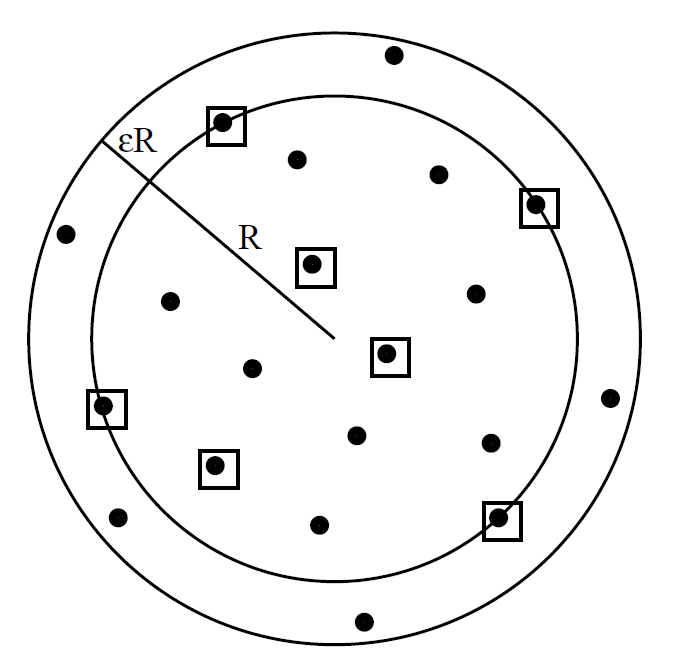
\includegraphics[width=0.3\textwidth]{figure/meb}
			\caption{最小闭包球问题,Badoiu et al. 通过迭代逐次拓展的方式,得到了该问题的$(1 + \epsilon)$近似解。}
		\end{figure}
		SVDD与MEB在数据只有一类标签时是统一的,其通过训练出一个最小的超球面,将这堆数据全部“包起来”,识别一个新的数据点时,如果这个数据点落在超球面内,就属于这个类,否则不是。
		MEB基于以下最小化问题:
		\begin{equation}
		\min R^{2}:\left\|\mathbf{c}-\phi\left(\mathbf{x}_{i}\right)\right\|^{2} \leq R^{2}, i=1, \ldots, m
		\end{equation}
		以下将其转换为对偶问题:
		$$
		\mathcal{L}(R, c, \alpha)= R^2 - \sum_{i=1}^{m}\alpha_{i}\left[R^2 - \parallel c - \phi(\mathbf{x}_{i})\parallel^2 \right]
		$$
		其中 $\alpha_{i} \geq 0, i = 1, \ldots, m$。对$\mathcal{L}(R, c, \alpha)$分别关于$R$, $c$求导,可得
		$$0=\nabla_{R} \mathcal{L}=2R(1-\sum_{i=1}^{m}\alpha_{i}) \Rightarrow \sum_{i=1}^{m}\alpha_{i} = 1$$
		$$
		\begin{aligned}
		0=\nabla_{c} \mathcal{L}= \nabla_{c}[R^2 - \sum_{i=1}^{m}\alpha_{i}&\left(c^T - \phi^T(\mathbf{x}_{i})\right) \left(c - \phi(\mathbf{x}_{i})\right) ] &\\\Rightarrow c = \sum_{i=1}^{m}\alpha_{i}\phi(\mathbf{x}_{i})
		\end{aligned}
		$$
		反代入$\mathcal{L}$, 整理得
		$$
		\begin{aligned} &\min _{R, C}\mathcal{L}(R, c, \alpha)= 
		R^2 - \sum_{i=1}^{m}\alpha_{i}\times\\&\left[R^2 - \left(\sum_{j=1}^{m}\alpha_{i}\phi^T(\mathbf{x}_{j}) - \phi^T(\mathbf{x}_{i})\right)\left(\sum_{k=1}^{m}\alpha_{i}\phi(\mathbf{x}_{k}) - \phi(\mathbf{x}_{i})\right)\right]\\&
		=\sum_{i=1}^{m}\alpha_{i}\left(\sum_{j=1}^{m}\alpha_{i}\phi^T(\mathbf{x}_{j}) - \phi^T(\mathbf{x}_{i})\right)\left(\sum_{k=1}^{m}\alpha_{i}\phi(\mathbf{x}_{k}) - \phi(\mathbf{x}_{i})\right) \\&
		=\sum_{i=1}^{m}\alpha_{i}\phi^T(\mathbf{x}_{i})\phi(\mathbf{x}_{i}) - \sum_{i,j=1}^{m}\alpha_{i}\alpha_{j}\phi^T(\mathbf{x}_{i})\phi(\mathbf{x}_{j}) \\&
		=\sum_{i=1}^{m} \alpha_{i} k\left(\mathbf{x}_{i}, \mathbf{x}_{i}\right)-\sum_{i, j=1}^{m} \alpha_{i} \alpha_{j} k\left(\mathbf{x}_{i}, \mathbf{x}_{j}\right)\end{aligned}
		$$
		可以得到最后的对偶问题,即参考文献[1]的第二式中的矩阵形式
		\begin{equation}
		\begin{aligned} \max _{\alpha_{i}} & \sum_{i=1}^{m} \alpha_{i} k\left(\mathbf{x}_{i}, \mathbf{x}_{i}\right)-\sum_{i, j=1}^{m} \alpha_{i} \alpha_{j} k\left(\mathbf{x}_{i}, \mathbf{x}_{j}\right) \\ \text { s.t. } & \alpha_{i} \geq 0, \quad i=1, \ldots, m \\ & \sum_{i=1}^{m} \alpha_{i}=1 \\ \max _{\alpha} \alpha^{\prime} &\operatorname{diag}(\mathbf{K})-\alpha^{\prime} \mathbf{K} \alpha : \alpha \geq 0, \alpha^{\prime} \textbf{1}=1 \end{aligned}
		\end{equation}
		$c$的解已经在前述给出,另解得$$
		R=\sqrt{\boldsymbol{\alpha}^{\prime} \operatorname{diag}(\mathbf{K})-\boldsymbol{\alpha}^{\prime} \mathbf{K} \boldsymbol{\alpha}}
		$$
		\subsubsection{CVM问题形式化}
		在 1.2.2 节已经说过,CVM 通过恰当的 kernel 形式,将 SVM 的原始问题求解转化为更适合高效迭代求解 MEB 问题。特别地,CVM 原论文作者发现,当满足 $k(\mathbf{x}, \mathbf{x})=\kappa$(常数) 时,可以得到 One-Class L2-SVM、Two-Class L2-SVM 与 MEB 对偶问题形式上的统一。
		\paragraph{One-Class L2-SVM}传统意义上,很多的分类问题试图解决两类或者多类情况,机器学习应用的目标是采用训练数据,将测试数据属于哪个类进行区分。但是如果只有一类数据,目标便是测试新的数据并且检测它是否与训练数据相似。方法是创建一个参数为 $\omega, b$ 的超平面,该超平面与特征空间中的零点距离最大,并且将零点与所有的数据点分隔开。参考论文[1]中将其加入了软间隔后的优化目标为:
		\begin{equation}
		\min _{\mathbf{\omega}, \rho, \xi_{i}}\|\mathbf{\omega}\|^{2}-2 \rho+C \sum_{i=1}^{m} \xi_{i}^{2}: \mathbf{\omega}^{\prime} \varphi\left(\mathbf{x}_{i}\right) \geq \rho-\xi_{i}
		\end{equation}
		同样地,将其写成拉格朗日乘子形式
		$$
		\mathcal{L}(\omega, \rho, \xi_i, \alpha)= \omega^T\omega - 2\rho + C\sum_{i=1}^{m}\xi_{i}^2 - 2\sum_{i=1}^{m}\alpha_{i}(\omega^T\phi(\mathbf{x}_{i}) - \rho + \xi_i)
		$$
		注意到这里拉格朗日乘子写作$2\alpha_{i}$不影响求解。
		$$0=\nabla_{\omega} \mathcal{L}=2\omega -2\sum_{i=1}^{m}\alpha_{i}\phi(\mathbf{x}_{i}) \Rightarrow \omega = \sum_{i=1}^{m}\alpha_{i}\phi(\mathbf{x}_{i})$$
		$$0=\nabla_{\rho} \mathcal{L}=-2 + 2\sum_{i=1}^{m}\alpha_{i} \Rightarrow \sum_{i=1}^{m}\alpha_{i} = 1$$
		$$0=\nabla_{\xi_i} \mathcal{L}=2C\sum_{i=1}^{m}\xi_i - 2\sum_{i=1}^{m}\alpha_{i} \Rightarrow \sum_{i=1}^{m}\xi_{i} = \frac{1}{C}$$
		回代(不再赘述了),可以得到最终形式
		\begin{equation}
		\begin{aligned} & \max -\boldsymbol{\alpha}^{\prime}\left(\mathbf{K}+\frac{1}{C} \mathbf{I}\right) \boldsymbol{\alpha}: 0 \leq \boldsymbol{\alpha}, \boldsymbol{\alpha}^{\prime} \mathbf{1}=1 \\=& \max -\boldsymbol{\alpha}^{\prime} \tilde{\mathbf{K}} \boldsymbol{\alpha}: 0 \leq \boldsymbol{\alpha}, \boldsymbol{\alpha}^{\prime} \mathbf{1}=1 \end{aligned}
		\end{equation}其中$
		\tilde{k}(\mathbf{z}, \mathbf{z})=\kappa+\frac{1}{C} \equiv \tilde{\kappa}, \tilde{\mathbf{K}}=\left[\tilde{k}\left(\mathbf{z}_{i}, \mathbf{z}_{j}\right)\right]
		$
		。这样,就完美地把单类别SVM问题转化成了在满足$k(\mathbf{x}, \mathbf{x})=\kappa$下的 MEB 最优解问题,即
		\begin{equation}
		\max -\boldsymbol{\alpha}^{\prime} \mathbf{K} \boldsymbol{\alpha}: 0 \leq \boldsymbol{\alpha}, \boldsymbol{\alpha}^{\prime} \mathbf{1}=1
		\end{equation}
		\paragraph{Two-Class L2-SVM}
		相似地,为了最优化
		\begin{equation}
		\begin{array}{cl}\min _{\mathbf{\omega}, b, \rho, \xi_{i}} & \|\mathbf{\omega}\|^{2}+b^{2}-2 \rho+C \sum_{i=1}^{m} \xi_{i}^{2} \\ \text { s.t. } & y_{i}\left(\mathbf{\omega}^{\prime} \varphi\left(\mathbf{x}_{i}\right)+b\right) \geq \rho-\xi_{i}\end{array}
		\end{equation}
		将其转化为对偶问题
		$$
		\begin{aligned} & \max _{0 \leq \alpha}-\alpha^{\prime}\left(\mathbf{K} \odot \mathbf{y y}^{\prime}+\mathbf{y y}^{\prime}+\frac{1}{C} \mathbf{I}\right) \boldsymbol{\alpha}: \alpha^{\prime} \mathbf{1}=1 \\=& \max -\boldsymbol{\alpha}^{\prime} \tilde{\mathbf{K}} \boldsymbol{\alpha}: 0 \leq \boldsymbol{\alpha}, \boldsymbol{\alpha}^{\prime} \mathbf{1}=1 \end{aligned}$$
		此处的 kernel 具体定义为$\tilde{k}\left(\mathbf{z}_{i}, \mathbf{z}_{j}\right)=y_{i} y_{j} k\left(\mathbf{x}_{i}, \mathbf{x}_{j}\right)+y_{i} y_{j}+\frac{\delta_{i j}}{C}$。读者可以自行验证,此处符合条件$k(\mathbf{x}, \mathbf{x})=$常量。\par
		由此,问题的所有形式化如上,我们已经在计算上证明了MEB 与 SVM 核函数满足一定条件下的等价性,这种条件并不严苛。事实上,许多很常见的核如高斯核,点积核,规范化核都是满足这个条件的,由此可以看出 CVM 架构的通用性。
		\subsubsection{CVM具体求解过程}
		以下为CVM算法框架,其中需要解释的是,在分类问题中Add\_Furthest\_Point使用了推导Two-Class L2-SVM得出的结论,从而有以下等价条件
		$$
		\begin{array}{l}\arg \max _{\mathbf{z_\ell} \notin B\left(\mathbf{c}_{t},(1+\epsilon) R_{t}\right)}\left\|\mathbf{c}_{t}-\tilde{\phi}\left(\mathbf{z}_{\ell}\right)\right\|^{2} \\ \quad=\arg \min _{\mathbf{z}_{\ell} \notin B\left(\mathbf{c}_{t},(1+\epsilon) R_{t}\right)} \sum_{\mathbf{z}_{i} \in {S}_{t}} \alpha_{i} y_{i} y_{\ell}\left(k\left(\mathbf{x}_{i}, \mathbf{x}_{\ell}\right)+1\right) \\ \quad=\arg \min _{\mathbf{z}_{\ell} \notin B\left(\mathbf{c}_{t},(1+\epsilon) R_{t}\right)} y_{\ell}\left(\mathbf{\omega}^{\prime} \phi\left(\mathbf{x}_{\ell}\right)+b\right)\end{array}
		$$
		\begin{algorithm}  
			\caption{Core Vector Machine}  
			\begin{algorithmic} %每行显示行号  
				\Require kernel $\tilde{k}$, 特征空间 $\tilde{\mathcal{F}}$, 映射$\tilde{\phi}$, 常数 $\tilde{\kappa}$
				\Ensure $c_B, R_B$, 核心集 $\mathcal{S}_{0}$
				\Function {Initialize}{$\tilde{\mathcal{F}}$, $\tilde{\phi}$}  
				\State 随机选取点 $z \in \tilde{\mathcal{F}}$
				\State 选取在 $\tilde{\mathcal{F}}$中离 $z$最远的点 $z_a$
				\State 选取在 $\tilde{\mathcal{F}}$中离 $z_a$最远的点 $z_b$
				
				\State$\begin{array}{l}R_{0}:=\frac{1}{2} \| \tilde{\phi}\left(\mathbf{z}_{a}\right)-  \tilde{\phi}\left(\mathbf{z}_{b}\right) \|\\=\frac{1}{2} \sqrt{\left\|\tilde{\phi}\left(\mathbf{z}_{a}\right)\right\|^{2}+\left\|\tilde{\phi}\left(\mathbf{z}_{b}\right)\right\|^{2}-2 \tilde{\phi}\left(\mathbf{z}_{a}\right)^{\prime} \tilde{\phi}\left(\mathbf{z}_{b}\right)}\\=  \frac{1}{2} \sqrt{2 \tilde{\kappa}-2 \tilde{k}\left(\mathbf{z}_{a}, \mathbf{z}_{b}\right)}\end{array}$
				\State $ \mathbf{c}_{0}:=\frac{1}{2}\left(\tilde{\phi}\left(\mathbf{z}_{a}\right)+\tilde{\phi}\left(\mathbf{z}_{b}\right)\right)$ 
				\State$
				{S}_{0}:=\left\{\mathbf{z}_{a}, \mathbf{z}_{b}\right\}
				$
				\State \Return{$R_{0}, {c}_{0}, {S}_{0}$}  
				\EndFunction  
				\State  
				\Function{Add\_Furthest\_Point}{$\tilde{\mathcal{F}}$, $\omega$, $b$,  $\phi$}
				\State \Return{$\arg \min _{\mathbf{z}_{\ell} \notin B\left(\mathbf{c}_{t},(1+\epsilon) R_{t}\right)} y_{\ell}\left(\mathbf{\omega}^{\prime} \phi\left(\mathbf{x}_{\ell}\right)+b\right)$}  
				\EndFunction 
				\State
				\Function{MEB}{$\tilde{\mathcal{F}}$, $\tilde{\phi}$, $S_{t+1}$}
				\State (With warm Start)
				\State $\alpha = SOLVE(QP problem in S_t)$
				\State $\mathbf{c}=\sum_{i=1}^{m} \alpha_{i} \tilde{\phi} \left(\mathbf{x}_{i}\right)$
				\State $R=\sqrt{\alpha^{\prime} \operatorname{diag}(\mathbf{K})-\alpha^{\prime} \mathbf{K} \alpha}$\ 
				\Return $\mathbf{c}, R $
				\EndFunction
				\State
				\Function{Main}{$\tilde{\mathcal{F}}$,$\tilde{k}$, $\tilde{\phi}$, $\tilde{\kappa}$}
				\State $R_{0}, {c}_{0}, {S}_{0}$ = \Call{Initialize}{$\tilde{\mathcal{F}}$, $\tilde{\phi}$} 
				$t = 0$
				\While{$\exists\ \tilde{\phi}(\mathbf{z})$不包含在$ B\left(\mathbf{c}_{t},(1+\epsilon) R_{t}\right)$中} 
				\State z = \Call{Add\_Furthest\_Point}{$\tilde{\mathcal{F}}$, $\omega$, $b$,  $\phi$} 
				\State $S_{t+1}={S}_{t} \cup\{\mathbf{z}\}$
				\State $\mathbf{c}_{t+1}, R_{t+1}=$ \Call{MEB}{$\tilde{\mathcal{F}}$, $\tilde{\phi}$, $S_{t+1}$}
				\State $t = t + 1$ 
				\EndWhile 
				\Return $c_B, R_B$
				\EndFunction 
				
			\end{algorithmic}  
		\end{algorithm}  
	\end{document}  
\paragraph{Paragraph} \lipsum[7] % Dummy text
\paragraph{Paragraph} \lipsum[8] % Dummy text
\begin{enumerate}[noitemsep] % [noitemsep] removes whitespace between the items for a compact look
	\item First item in a list
	\item Second item in a list
	\item Third item in a list
\end{enumerate}

\subsection{Subsection}

\lipsum[9] % Dummy text

\begin{figure}[ht]\centering
\includegraphics[width=\linewidth]{results}
\caption{In-text Picture}
\label{fig:results}
\end{figure}

Reference to Figure \ref{fig:results}.

%------------------------------------------------

\section{Results and Discussion}

\lipsum[10] % Dummy text

\subsection{Subsection}

\lipsum[11] % Dummy text

\begin{table}[hbt]
\caption{Table of Grades}
\centering
\begin{tabular}{llr}
\toprule
\multicolumn{2}{c}{Name} \\
\cmidrule(r){1-2}
First name & Last Name & Grade \\
\midrule
John & Doe & $7.5$ \\
Richard & Miles & $2$ \\
\bottomrule
\end{tabular}
\label{tab:label}
\end{table}

\subsubsection{Subsubsection}

\lipsum[12] % Dummy text

\begin{description}
\item[Word] Definition
\item[Concept] Explanation
\item[Idea] Text
\end{description}

\subsubsection{Subsubsection}

\lipsum[13] % Dummy text

\begin{itemize}[noitemsep] % [noitemsep] removes whitespace between the items for a compact look
\item First item in a list
\item Second item in a list
\item Third item in a list
\end{itemize}

\subsubsection{Subsubsection}

\lipsum[14] % Dummy text

\subsection{Subsection}

\lipsum[15-23] % Dummy text

%------------------------------------------------
\phantomsection
\section*{Acknowledgments} % The \section*{} command stops section numbering

\addcontentsline{toc}{section}{Acknowledgments} % Adds this section to the table of contents

So long and thanks for all the fish \cite{Figueredo:2009dg}.

%----------------------------------------------------------------------------------------
%	REFERENCE LIST
%----------------------------------------------------------------------------------------

\phantomsection
\bibliographystyle{unsrt}
\bibliography{}
[1] Ivor W. Tsang, James T. Kwok, Pak-Ming Cheung: Core Vector Machines: Fast SVM
Training on Very Large Data Sets. J. Mach. Learn. Res. 6: 363-392 ,2005.\\ \ 
[2] Gaëlle Loosli, Stéphane Canu: Comments on the "Core Vector Machines: Fast SVM
Training on Very Large Data Sets". J. Mach. Learn. Res. 8: 291-301 ,2007.\\ \
[3] Ivor W. Tsang, James T. Kwok, and Pak-Ming Cheung. Very large SVM training using
Core Vector Machines. In Proceedings of the Tenth International Workshop on Artificial
Intelligence and Statistics (AISTAT’05). Society for Artificial Intelligence and Statistics,
2005.\\ \ 
[4] Badoiu, M., \& Clarkson, K. (2002). Optimal core-sets for balls.
DIMACS Workshop on Computational Geometry.

%----------------------------------------------------------------------------------------

\end{document}